\documentclass[5p]{elsarticle}
\usepackage{graphicx}

\begin{document}
\begin{frontmatter}
\title{An overview of the Data for Jooriland\tnoteref{t1}}
\tnotetext[t1]{This document is designed to provide a quick overview of the data.}
\author[jsl]{Jason Lessels}
\address[jsl]{The University of Sydney}
\ead{j.lessels@usyd.edu.au}
\begin{abstract}
This article is designed to provide an overview of the data being used to optimise the sampling scheme currently used by the SCA. Current
\end{abstract}
\begin{keyword}
\end{keyword}

\end{frontmatter}
\section*{Introduction}
Water quality sampling is common place and required by law to allow catchment management agentcies to maintain the health of a catchment. It is now well established that Australian streams have the highest levels of nutrient exports during storm events. Due to this relationship, sampling schemes are currently shifting from a monthly sampling basis, to a event-based sampling scheme. The shift has caused a necessary shift in the statistics that are currently used to analyses the data.

The data obtained from the Sydeny Catchment Authority (SCA) has a continuos discharge data set starting early 1960 and ending in 2009. The water quality dataset currently being used was supplied mid 2008. This dataset starts in 1991 and ends in 2008. This dataset is heavily biased with the starting of this dataset, being only collected via routine and flood, samples. This bias leads to the belief that the data in the early part of the data set has missed several key events.
\section*{Background}
The Sydney Catchment Authority is in charge of the drinking water for the metropolitan area of Sydney. The catchment is a large catchment, that streches from Gouldburn in the South to Bathurst in the North. The catchment is characteried by low lying hills in the south, which is dryer th...

\section*{Data Summary}
The data collected from the SCA covers a variety of variables. This paper will only cover EC,TP,TN,and NTU variables. An overivew of the data is provided in table \ref{table:summary_stats}. Correlation plots between the variables are also provided in figure \ref{fig:correlation_plots}. The correlation plots provide an overview of the relationships between the various water quality variables and the assoicated discharge.

% Fri Nov 20 13:04:05 2009
\begin{table}[ht]
\begin{center}
\caption{Summary statistics of data}
\begin{tiny}
\begin{tabular}{rrrrrrr}
  \hline
Statistic & pH & EC & NTU & TN & TP & Discharge \\ 
  \hline
Min & 6.50 & 0.02 & 0.54 & 0.17 & 0.00 & 0.00 \\ 
  Max & 9.16 & 0.71 & 1000.00 & 14.80 & 2.28 & 2507.99 \\ 
  Mean & 7.84 & 0.29 & 67.43 & 0.87 & 0.07 & 163.40 \\ 
  Median & 7.80 & 0.30 & 15.70 & 0.60 & 0.02 & 42.03 \\ 
  Stdev & 0.53 & 0.11 & 140.88 & 1.00 & 0.15 & 335.10 \\ 
  n & 285.00 & 1125.00 & 1314.00 & 523.00 & 513.00 & 1375.00 \\ 
   \hline
\end{tabular}
\end{tiny}
\label{table:summary_stats}
\end{center}
\end{table}
The samples of the water quality variables have been collected using a variety of methods. These methods are summarised in table \ref{table:sample_types}

\begin{table}[ht]
\begin{center}
\caption{Quanity of sample types in relation to water quality variable}
\begin{tabular}{lrrrrr}
  \hline
 Sample type & pH & EC & TP & TN & NTU \\ 
  \hline
  unknown &  60 &   0 & 128 & 128 & 120 \\ 
  automatic &  25 & 850 & 121 & 124 & 926 \\ 
  composite &   1 &  35 &  25 &  31 &  35 \\ 
  duplicate &   3 &   3 &   4 &   4 &   3 \\ 
  flood &   0 &  22 &  19 &  18 &  18 \\ 
  N &   0 &   0 &   0 &   0 &   0 \\ 
  monthly grab & 166 & 167 & 168 & 168 & 165 \\ 
  ad-hoc grab &  30 &  39 &  38 &  40 &  38 \\ 
  W &   0 &   9 &  10 &  10 &   9 \\ 
   \hline
\end{tabular}
\label{table:sample_types}
\end{center}
\end{table}


\begin{center}
\begin{figure}
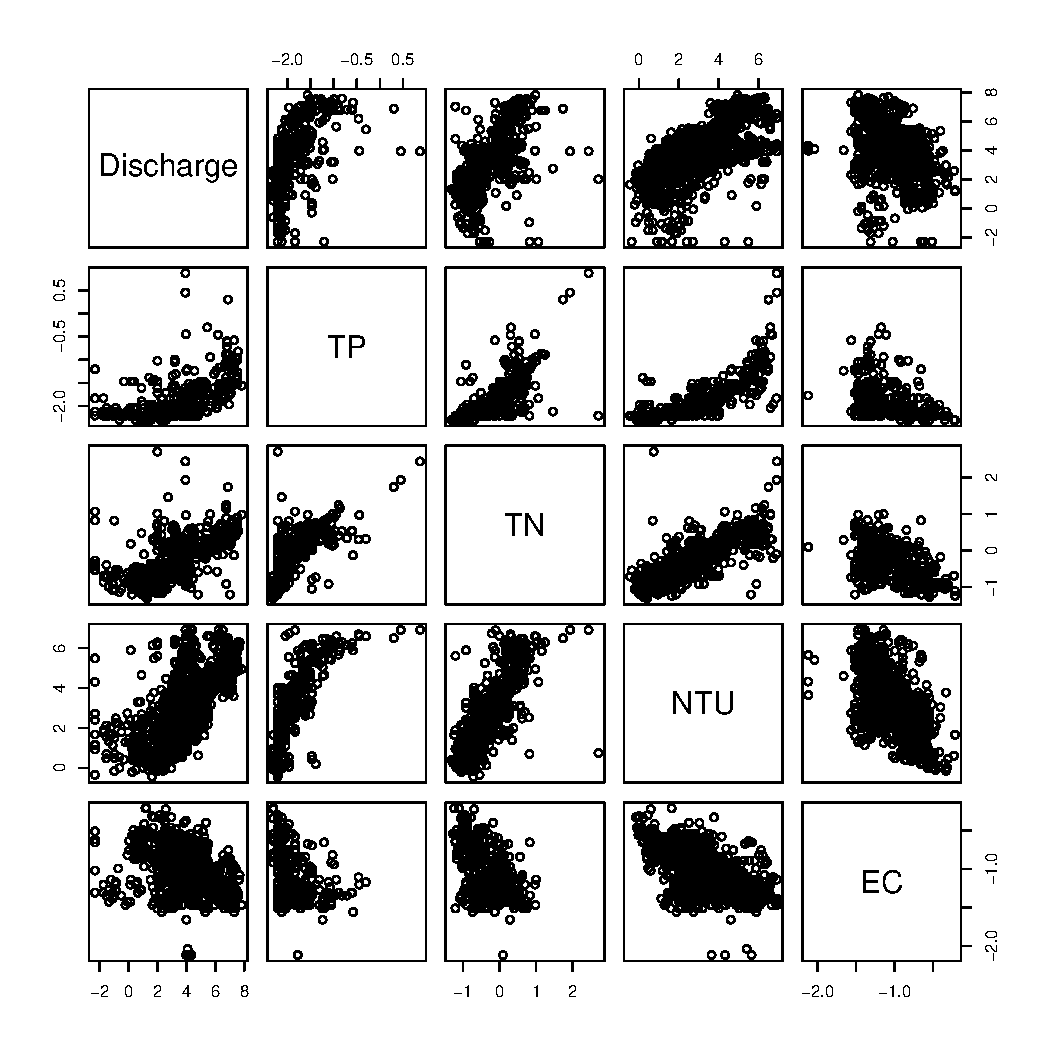
\includegraphics[scale=0.50]{Scatterplotmatrix.pdf}
\caption{Scatter plot of water quality variables.\it{All variables are log transformed.}}
\label{fig:correlation_plots}
\end{figure}
\end{center}



\pagebreak
\section*{Current statistics}


\end{document} 
